%
% strahlung.tex
%
% (c) 2025 Prof Dr Andreas Müller
%
\documentclass[tikz]{standalone}
\usepackage{amsmath}
\usepackage{times}
\usepackage{txfonts}
\usepackage{pgfplots}
\usepackage{csvsimple}
\usetikzlibrary{arrows,intersections,math}
\begin{document}
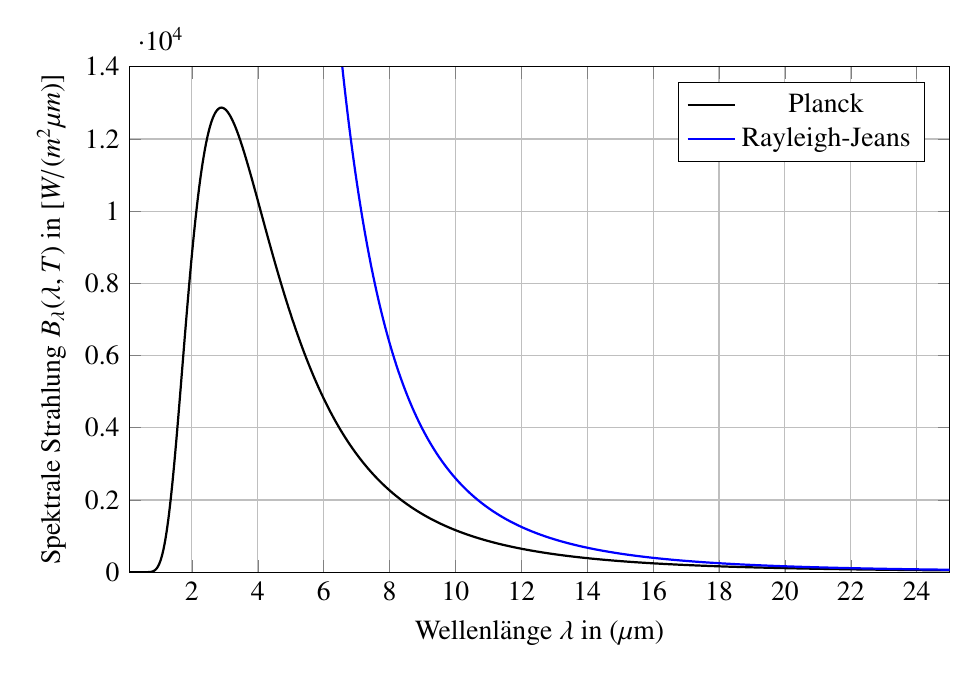
\begin{tikzpicture}
% Hauptachse (linke y-Achse; Werte von 0 bis 14000)
\begin{axis}[
	name=leftaxis,
	width=12cm,
	height=8cm,
	xlabel={Wellenlänge $\lambda$ in ($\mu$m)},
	ylabel={Spektrale Strahlung $B_\lambda(\lambda, T)$ in $[W/(m^2 \mu m)]$},
	xmin=0.1, xmax=25,
	ymin=0, ymax=14000,
	legend style={at={(0.97,0.97)}, anchor=north east},
	grid=both,
	domain=0.01:26,
	samples=1000
	]
	%W\,m$^{-2}$m$^{-1}
	% Konstanten (SI)
	\def\h{6.62607015e-34}       % Plancksche Konstante
	\def\c{2.99792458e8}         % Lichtgeschwindigkeit
	\def\kB{1.380649e-23}        % Boltzmann-Konstante
	\def\T{1000}                 % Temperatur in Kelvin
	
	% --- Plancksche Strahlungsformel ---
	\addplot[black, thick] 
	expression{
		(2*pi*\h*\c^2)/((x*1e-6)^5) * 1/(exp(\h*\c/((x*1e-6)*\kB*\T)) - 1) / 1e6
	};
	\addlegendentry{Planck}
	
	
	% --- Rayleigh-Jeans-Gesetz (Langwellennähe) ---
	\addplot[blue, thick, restrict y to domain=0:14000]
	expression{
		(2*pi*\c*\kB*\T)/((x*1e-6)^4) / 1e6
	};
	\addlegendentry{Rayleigh-Jeans}
\end{axis}
\end{tikzpicture}
\end{document}

